%---------------------------------------------------------------------
\section{Cross-Check Samples}
\label{data-MC}

A crucial step in the single top search is to establish that the
background model is appropriate while minimizing looking into the
search region. For this purpose, two background-dominated control
samples are defined, and a comparison between the 1D discriminants in
data and the background model is performed.

These two control samples are selected by applying the standard event
selection, and requiring in addition $H_T<175$~GeV and $H_T>300$~GeV,
respectively. Two-jet events are largely dominated by $W$+jets
events, and thus it is the modeling of this background that is mainly
addressed by these cross checks. We refer to these control samples as
``soft $W$+jets'' and ``hard $W$+jets'' respectively. In the case of
three-jet events, the ``hard $W$+jets'' sample also contains a
significant fraction of $\ttbar$.

The ``soft $W$+jets'' sample selects low momentum $W$+jets and
multijets events and almost no top-quark events.
Figures~\ref{wjets-cross-2jet} and \ref{wjets-cross-3jet} compare the
$tb$ and $tq$ discriminants between data and the background model for
events with two and three jets respectively. Good agreement is seen
between data and expectation.

The ``hard $W$+jets'' sample selects mainly $\ttbar$ and high momentum
$W$+jets events. Figures~\ref{ttbar-cross-2jet} and
\ref{ttbar-cross-3jet} compare the $tb$ and $tq$ discriminants between
data and the background model for events with two and three jets. Good
agreement is again found between data and expectation.

Most of the signal, and thus the problematic $W$+jets background, has
$H_T$ between these cuts. Therefore, by confirming that the observed
discriminant distribution is well reproduced by the background model
for the softest and hardest $W$+jets events, we gain confidence that
the $W$+jets background in the signal region is also well modeled.

\clearpage

\begin{figure}[!h!tbp]
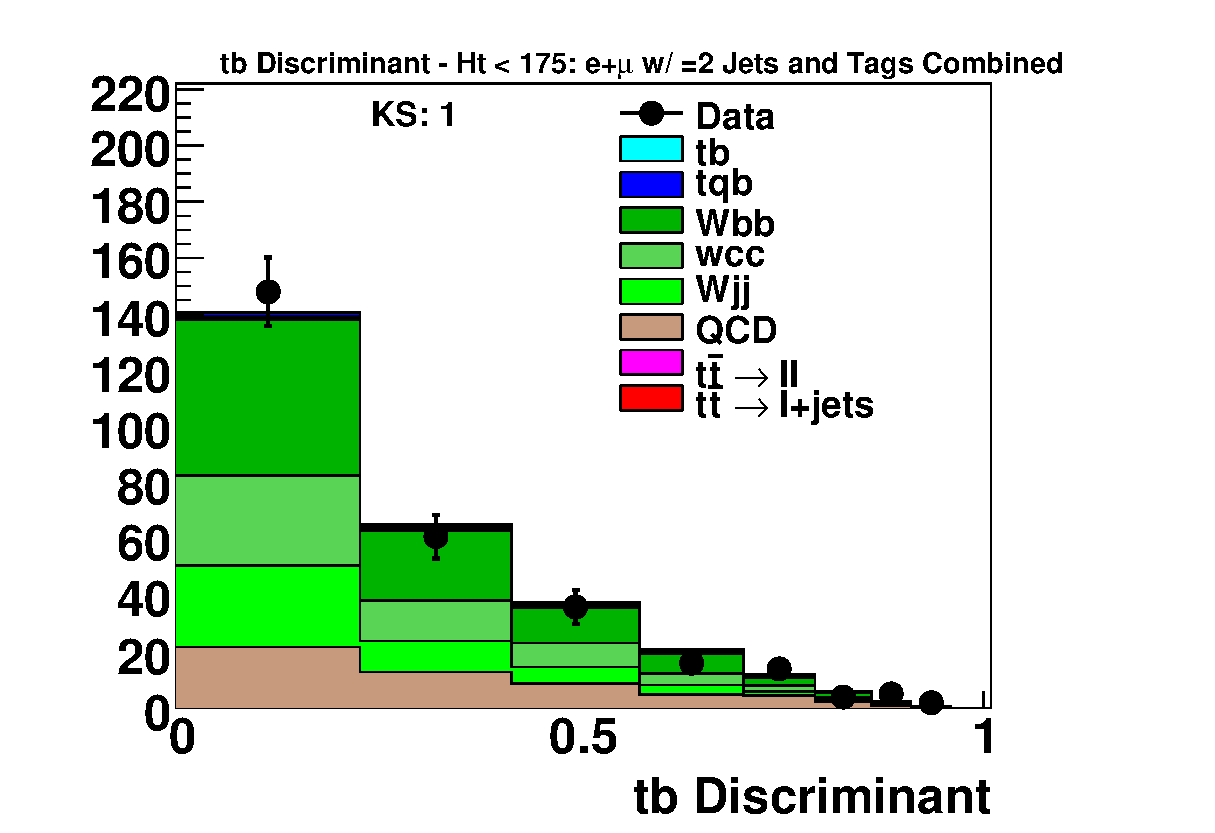
\includegraphics[width=0.40\textwidth]
{figures/cross_check/combined/2jet/Wjets_tb_Discriminant}
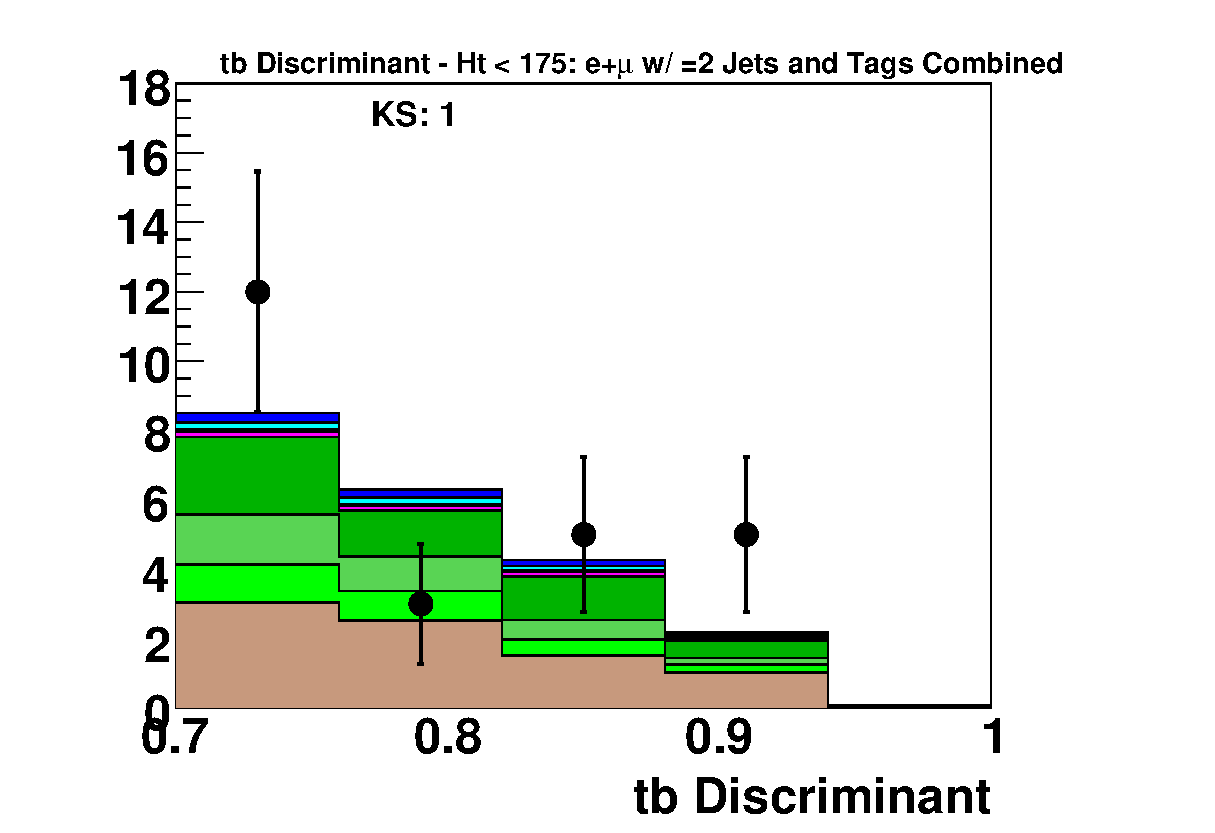
\includegraphics[width=0.40\textwidth]
{figures/cross_check/combined/2jet/Wjets_tb_Discriminant_Zoom}
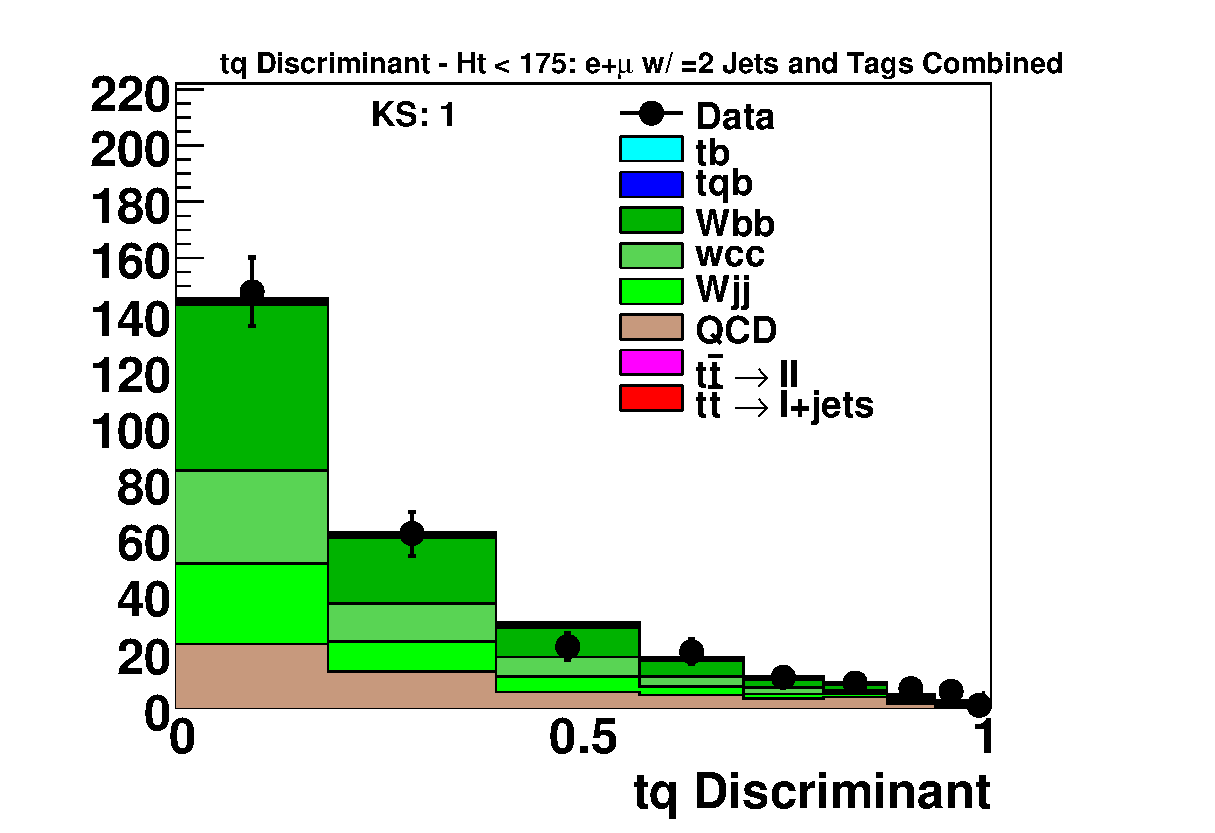
\includegraphics[width=0.40\textwidth]
{figures/cross_check/combined/2jet/Wjets_tq_Discriminant}
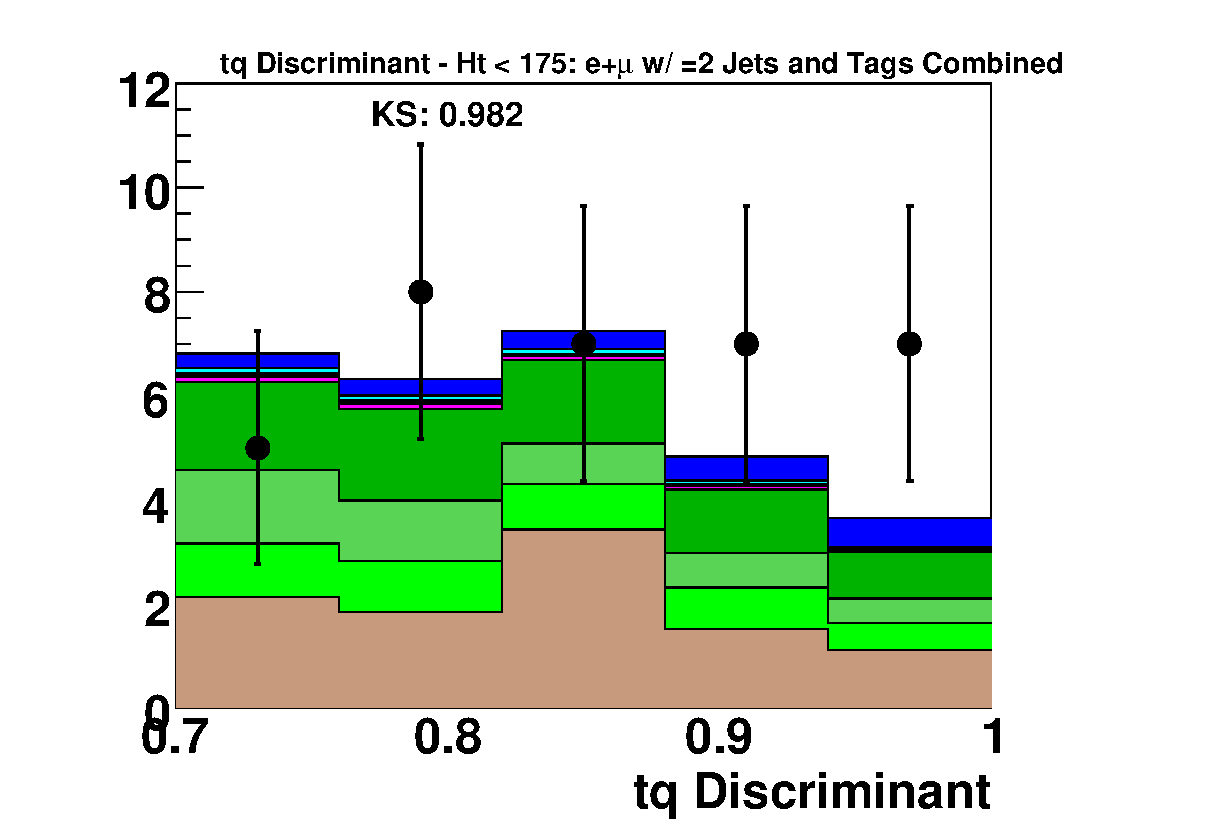
\includegraphics[width=0.40\textwidth]
{figures/cross_check/combined/2jet/Wjets_tq_Discriminant_Zoom}
\vspace{-0.1in}
\caption[wjetscross]{``Soft $W$+jets'' cross-check plots in two-jet
events for the $tb$ discriminant (upper row) and the $tq$ discriminant
(lower row). The left column shows the full discriminant region while
the right column shows the high discriminant region above 0.7.}
\label{wjets-cross-2jet}
\end{figure}

\begin{figure}[!h!tbp]
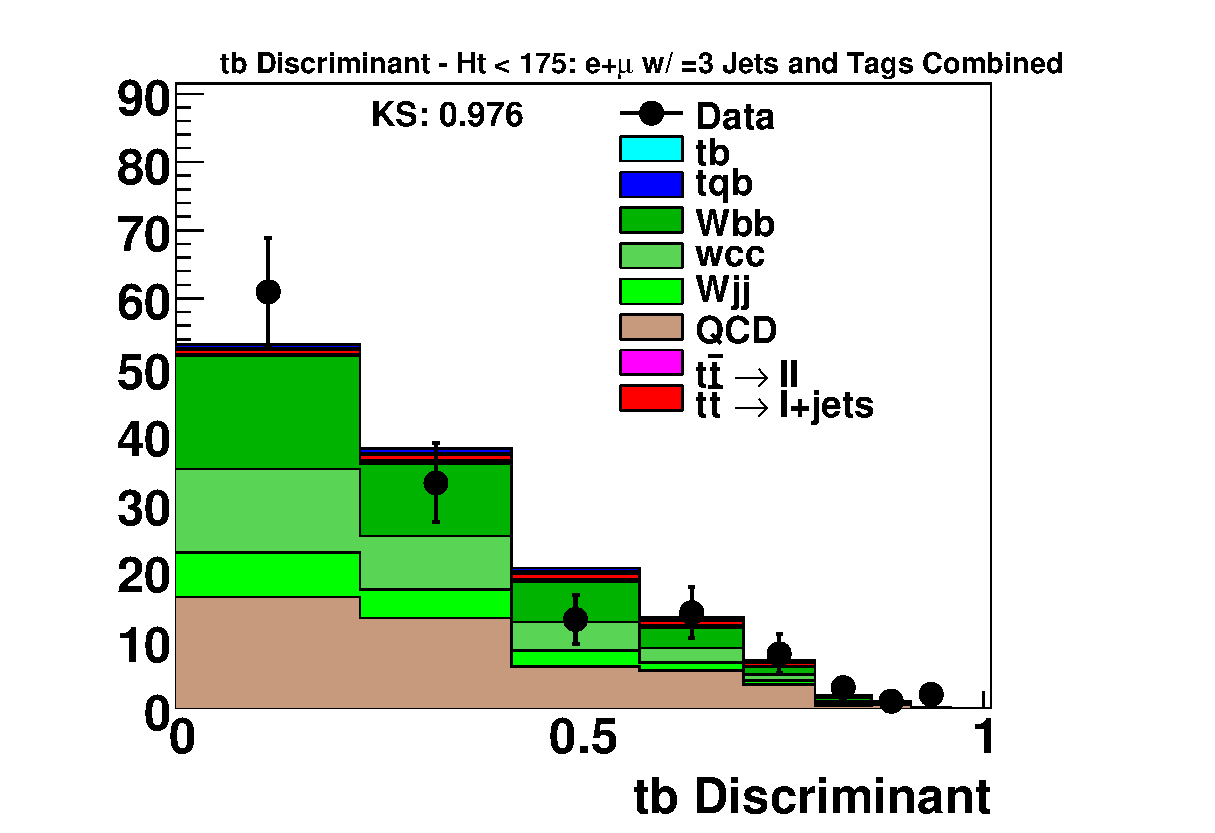
\includegraphics[width=0.40\textwidth]
{figures/cross_check/combined/3jet/Wjets_tb_Discriminant}
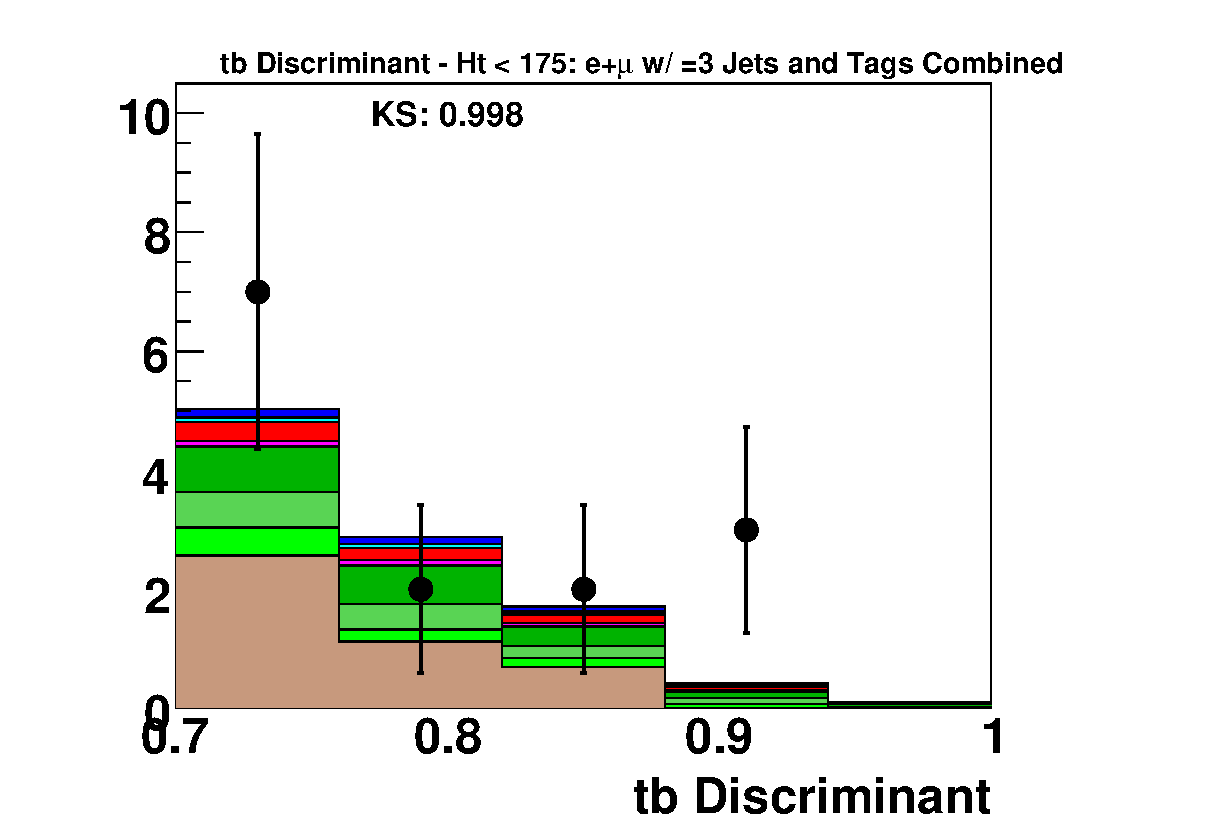
\includegraphics[width=0.40\textwidth]
{figures/cross_check/combined/3jet/Wjets_tb_Discriminant_Zoom}
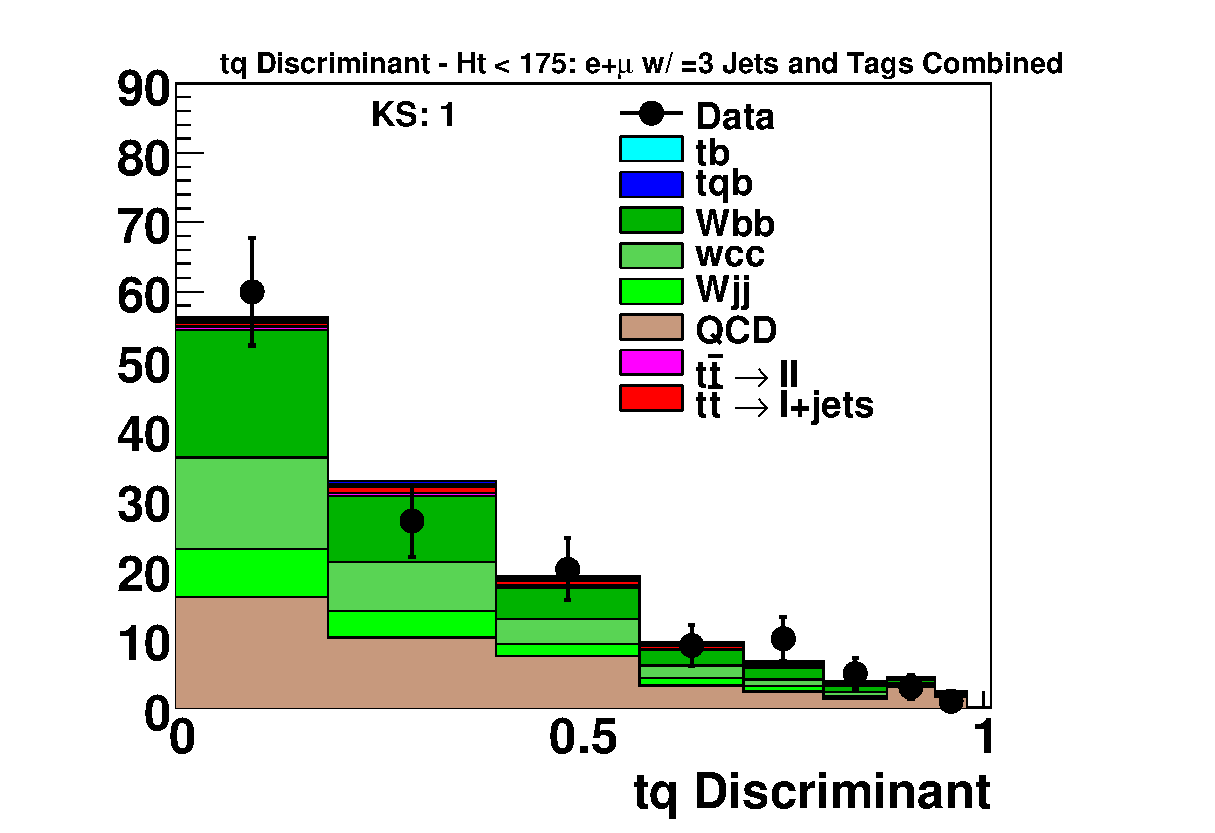
\includegraphics[width=0.40\textwidth]
{figures/cross_check/combined/3jet/Wjets_tq_Discriminant}
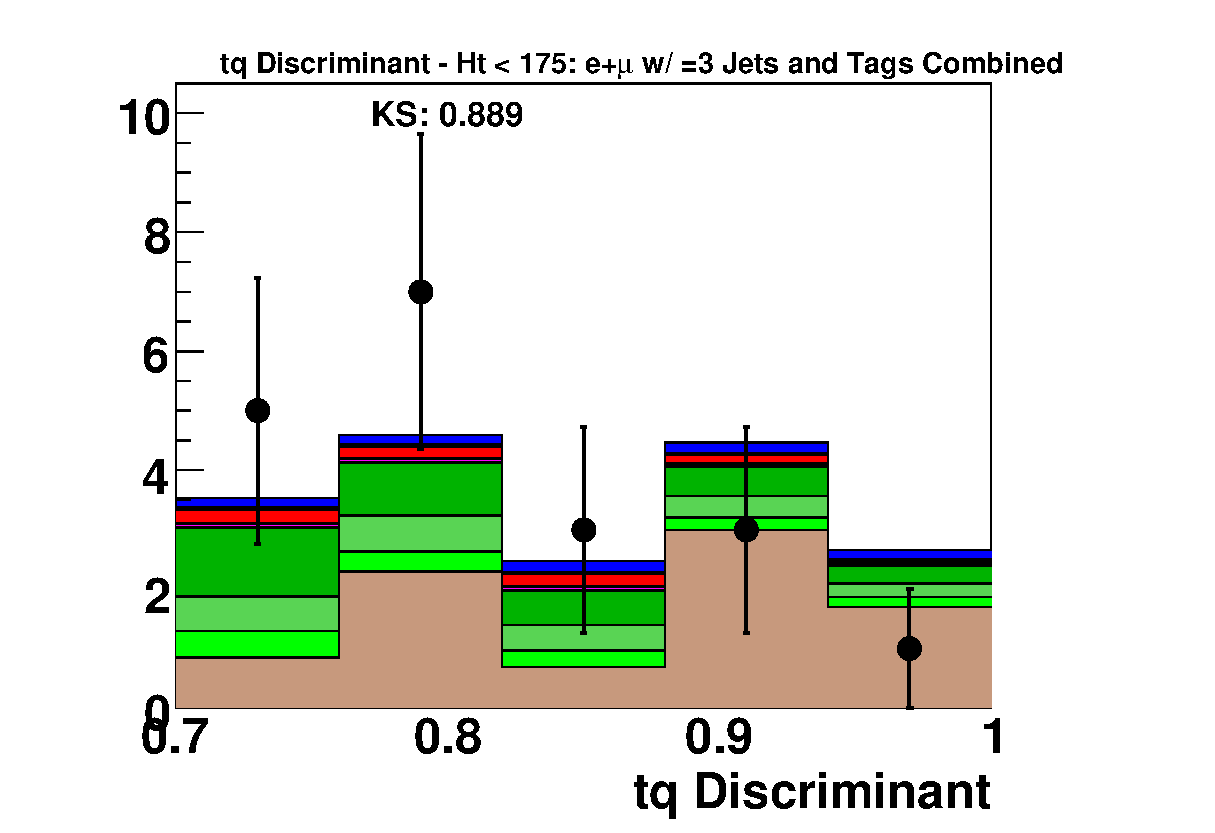
\includegraphics[width=0.40\textwidth]
{figures/cross_check/combined/3jet/Wjets_tq_Discriminant_Zoom}
\vspace{-0.1in}
\caption[wjetscross]{``Soft $W$+jets'' cross-check plots in three-jet
events for the $tb$ discriminant (upper row) and the $tq$ discriminant
(lower row). The left column shows the full discriminant region while
the right column shows the high discriminant region above 0.7.}
\label{wjets-cross-3jet}
\end{figure}

\begin{figure}[!h!tbp]
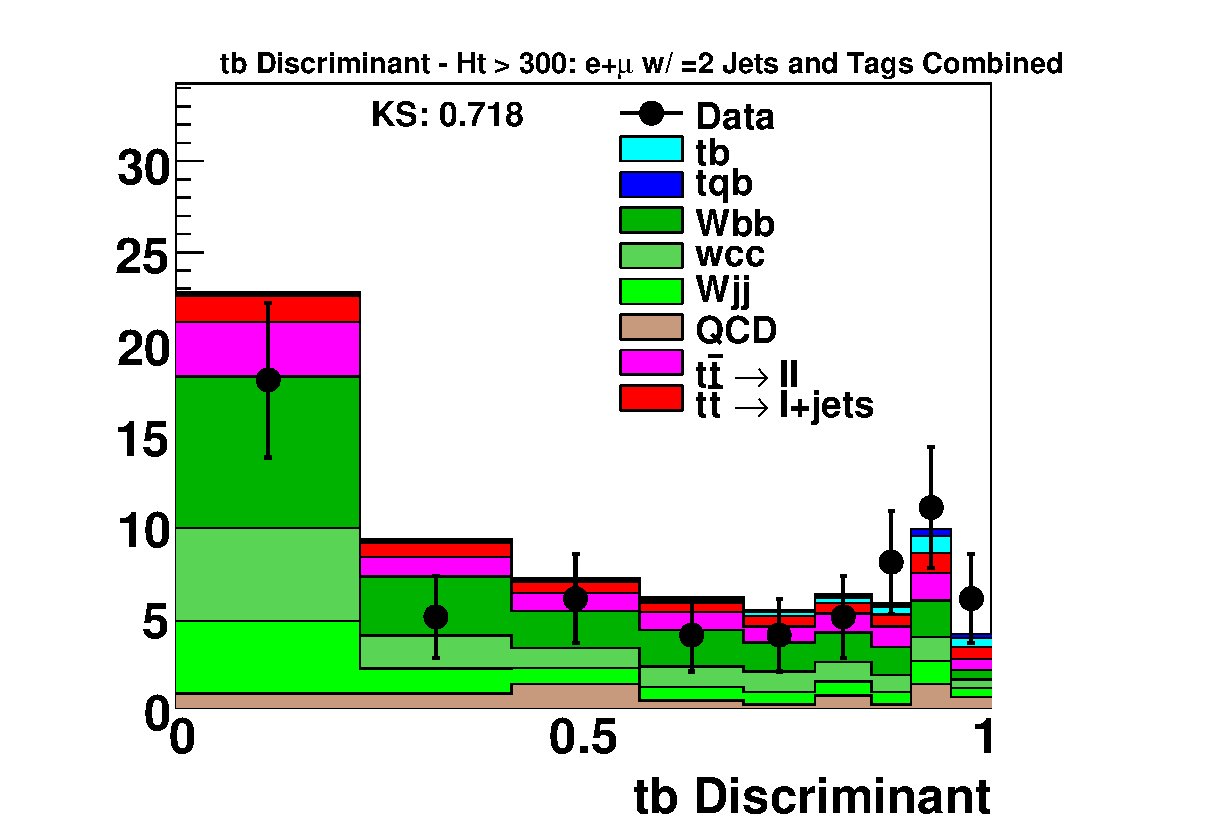
\includegraphics[width=0.40\textwidth]
{figures/cross_check/combined/2jet/TTbar_tb_Discriminant}
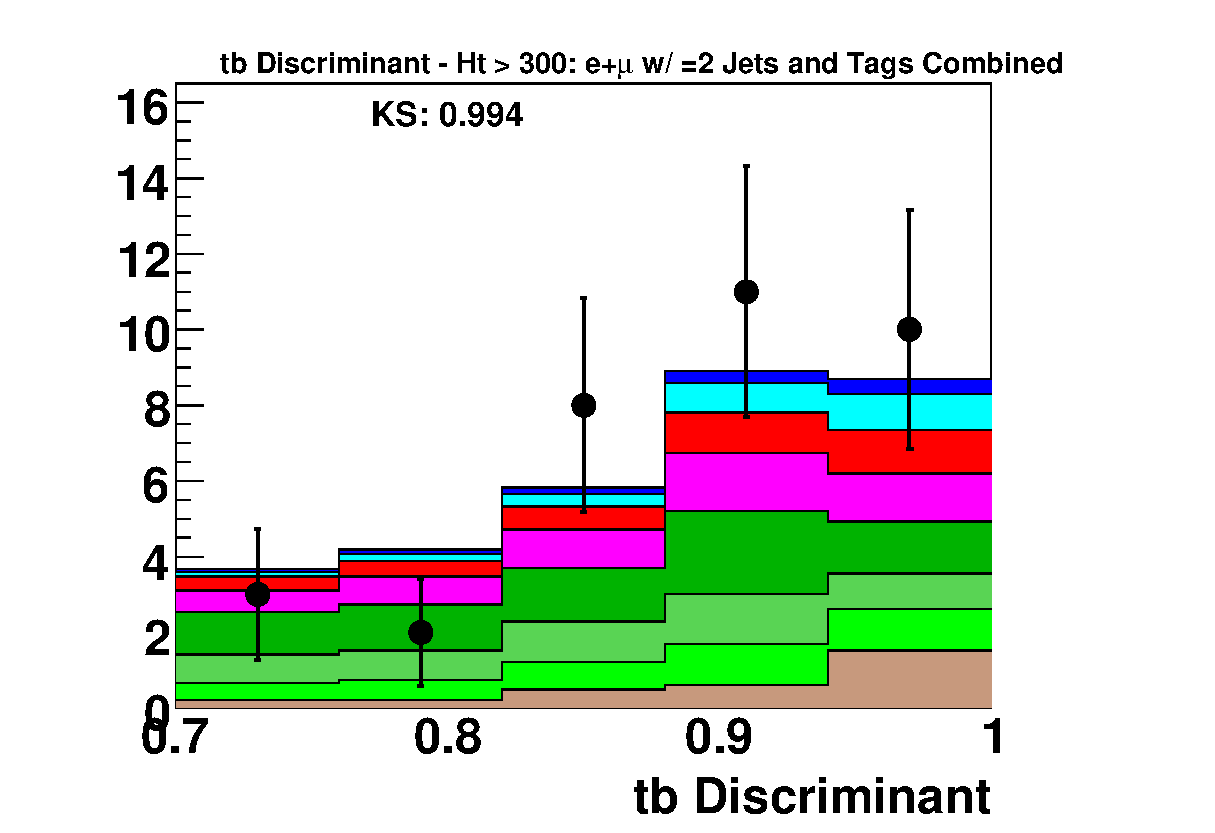
\includegraphics[width=0.40\textwidth]
{figures/cross_check/combined/2jet/TTbar_tb_Discriminant_Zoom}
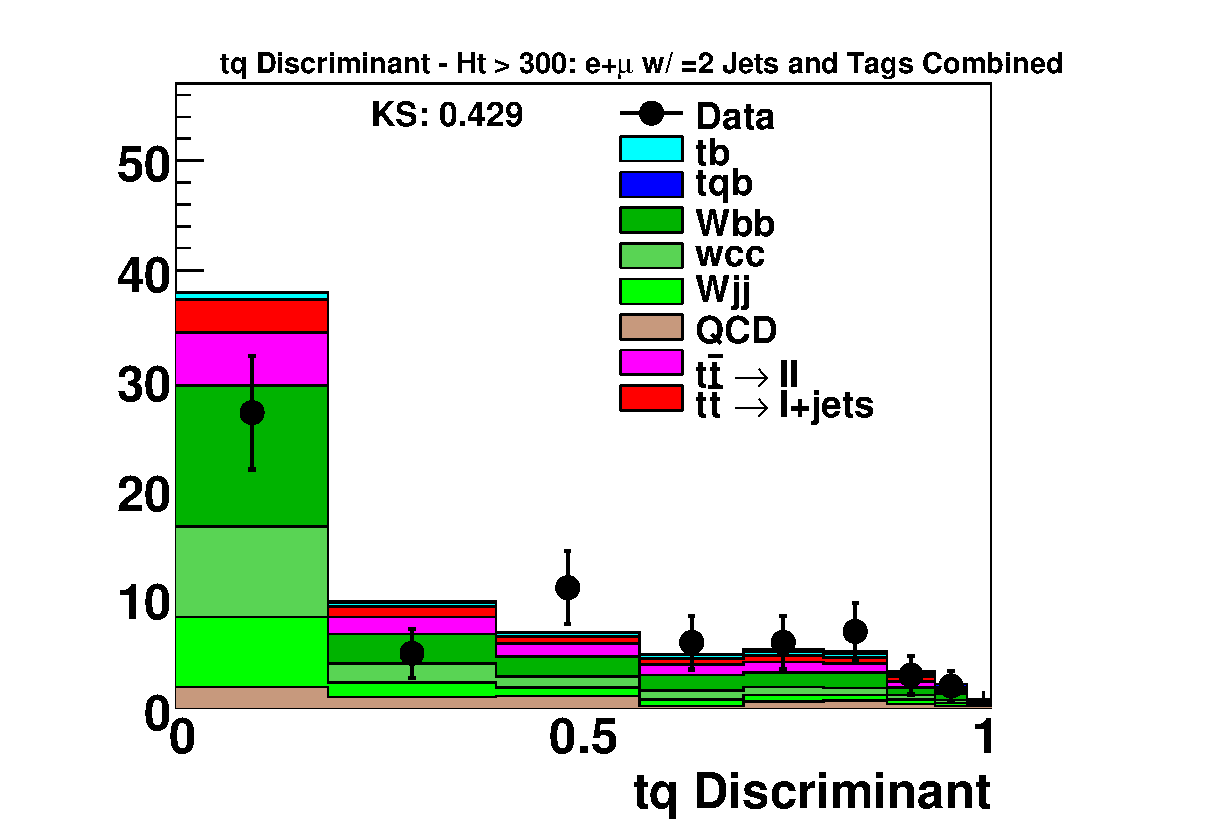
\includegraphics[width=0.40\textwidth]
{figures/cross_check/combined/2jet/TTbar_tq_Discriminant}
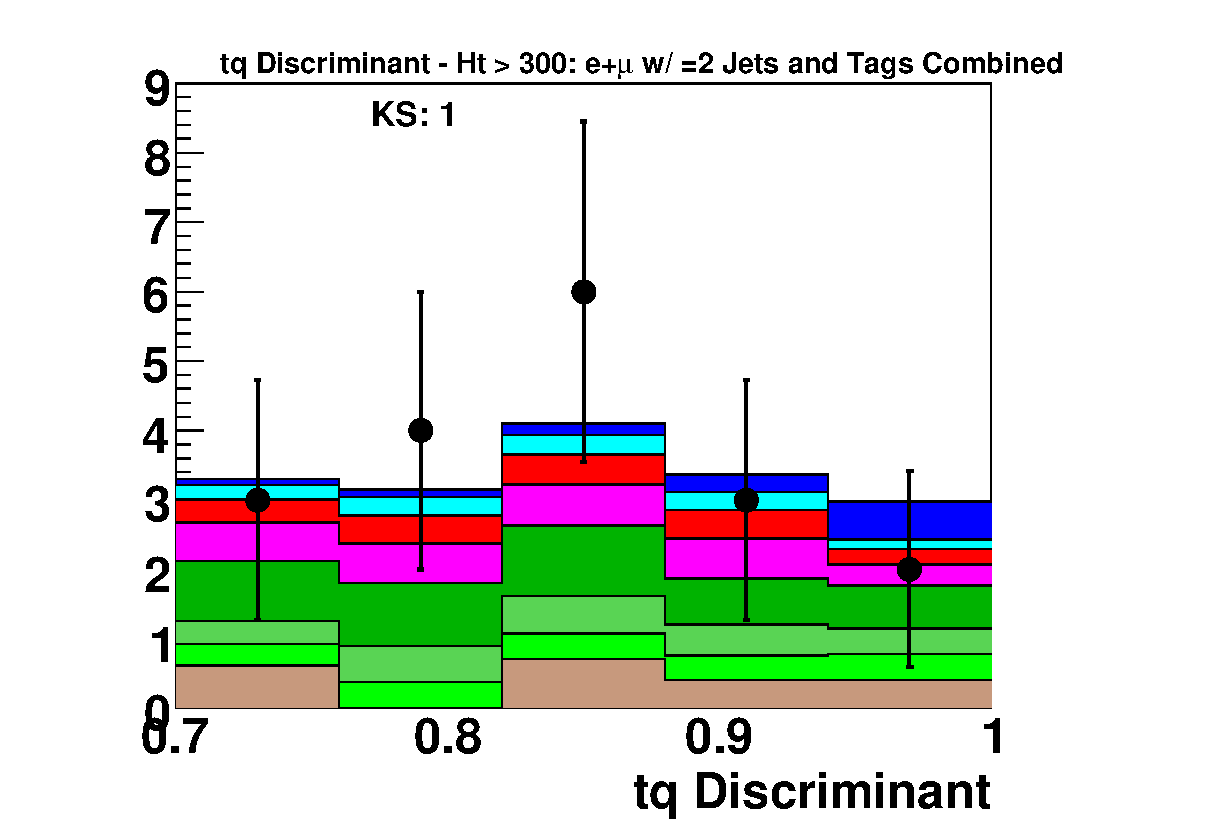
\includegraphics[width=0.40\textwidth]
{figures/cross_check/combined/2jet/TTbar_tq_Discriminant_Zoom}
\vspace{-0.1in}
\caption[ttbarcross]{``Hard $W$+jets'' cross-check plots in two-jet
events for the $tb$ discriminant (upper row) and the $tq$ discriminant
(lower row). The left column shows the full discriminant region while
the right column shows the high discriminant region above 0.7.}
\label{ttbar-cross-2jet}
\end{figure}

\begin{figure}[!h!tbp]
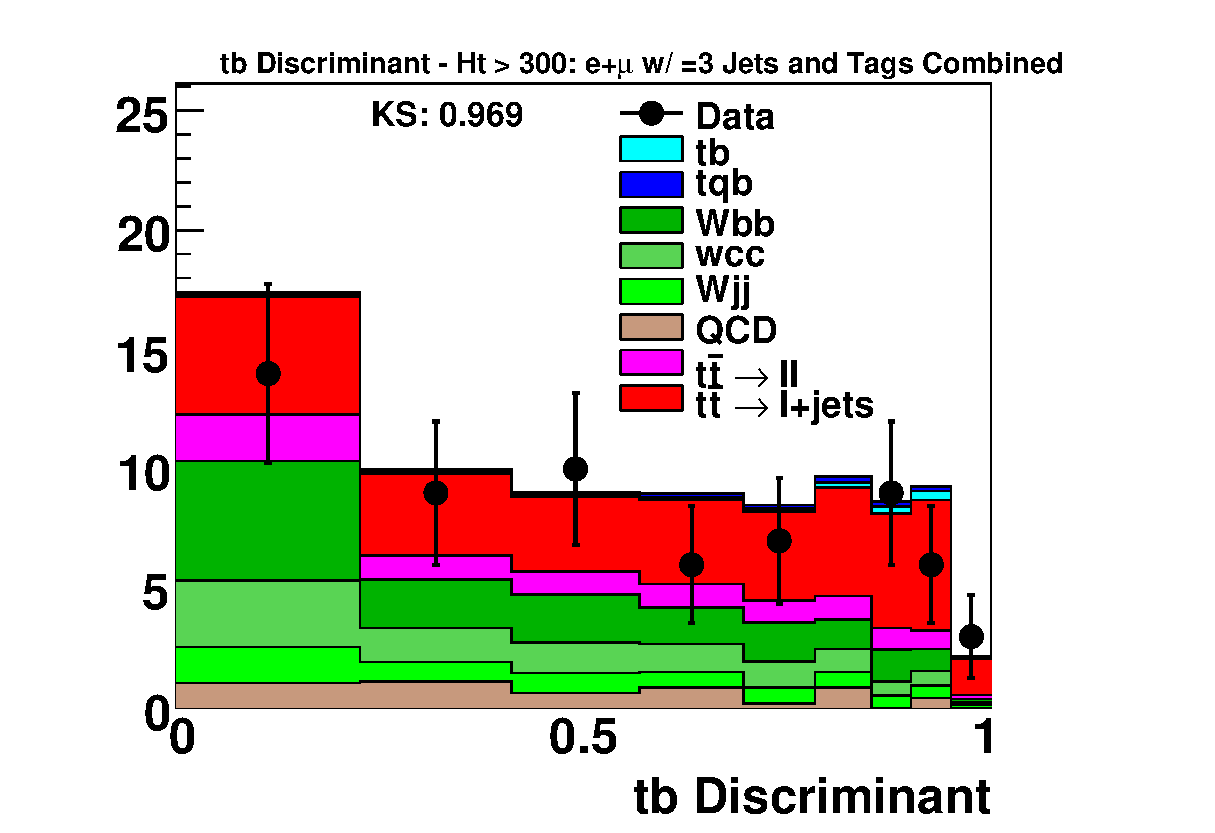
\includegraphics[width=0.40\textwidth]
{figures/cross_check/combined/3jet/TTbar_tb_Discriminant}
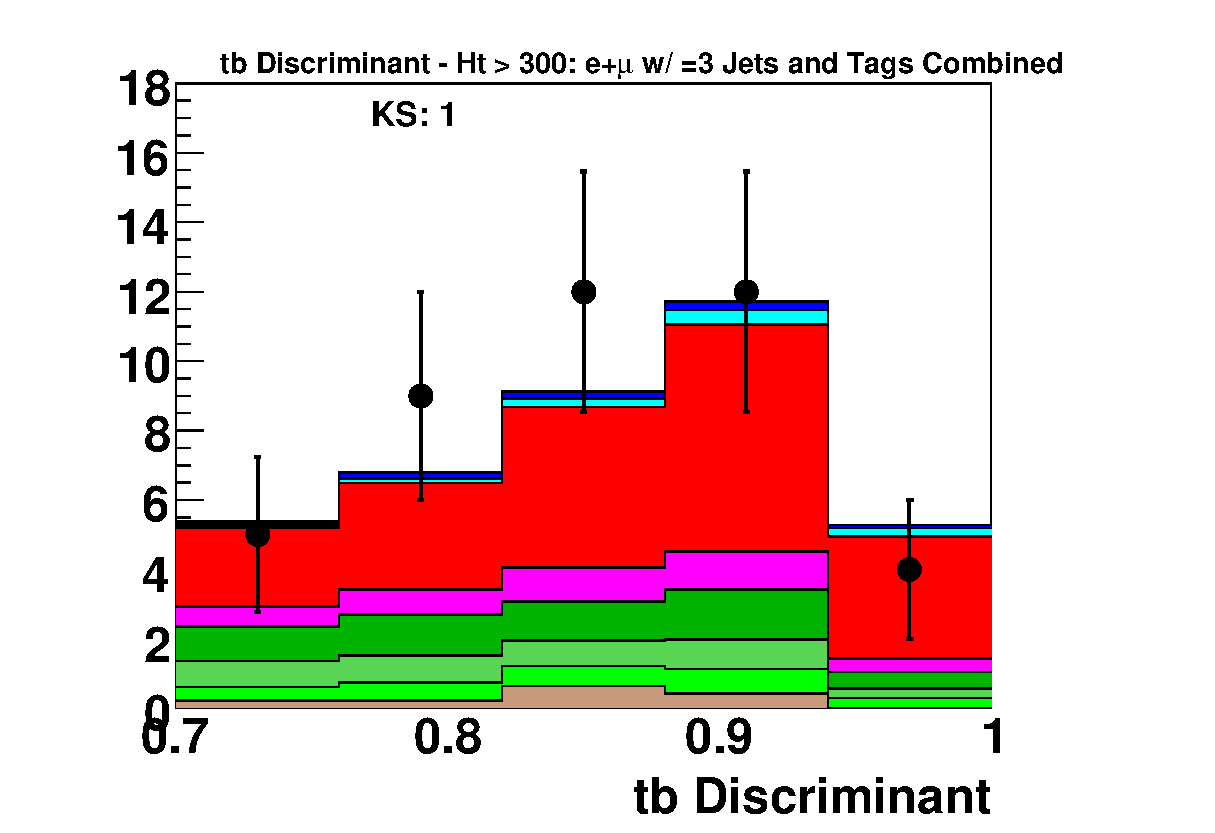
\includegraphics[width=0.40\textwidth]
{figures/cross_check/combined/3jet/TTbar_tb_Discriminant_Zoom}
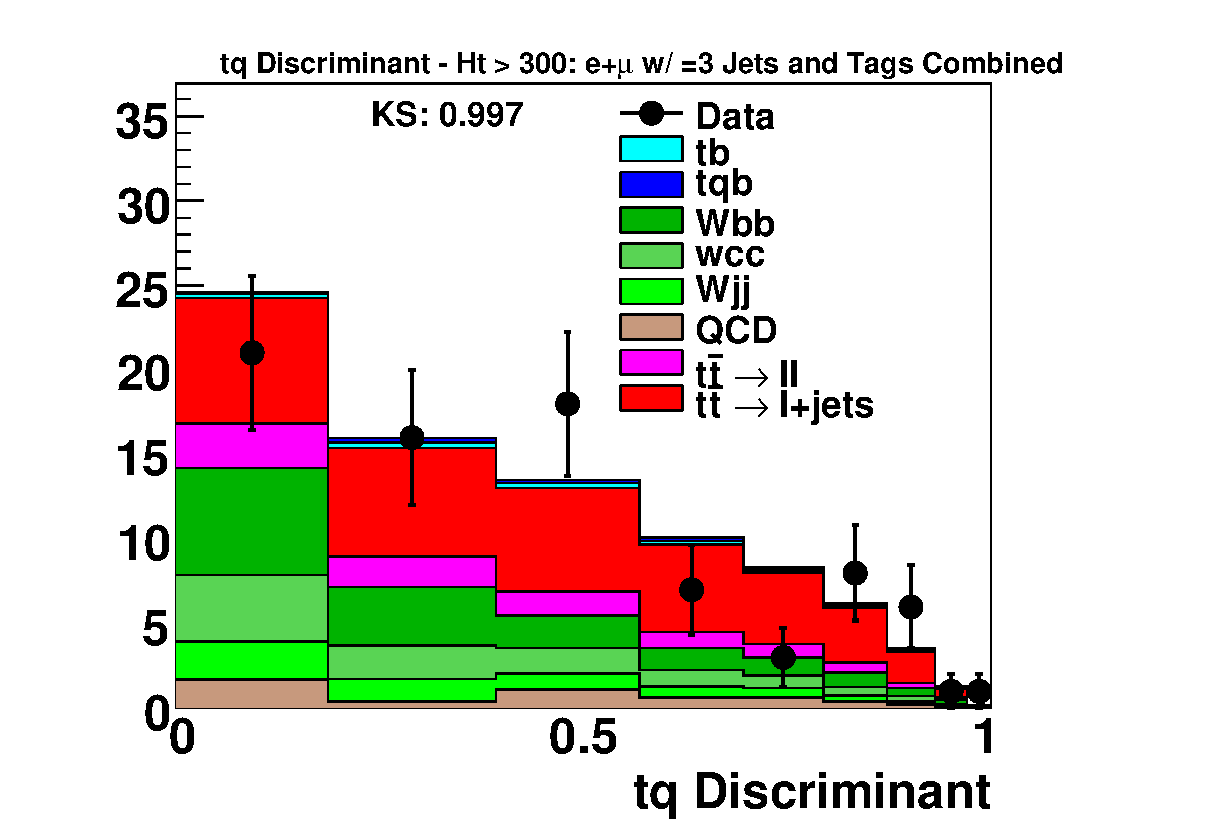
\includegraphics[width=0.40\textwidth]
{figures/cross_check/combined/3jet/TTbar_tq_Discriminant}
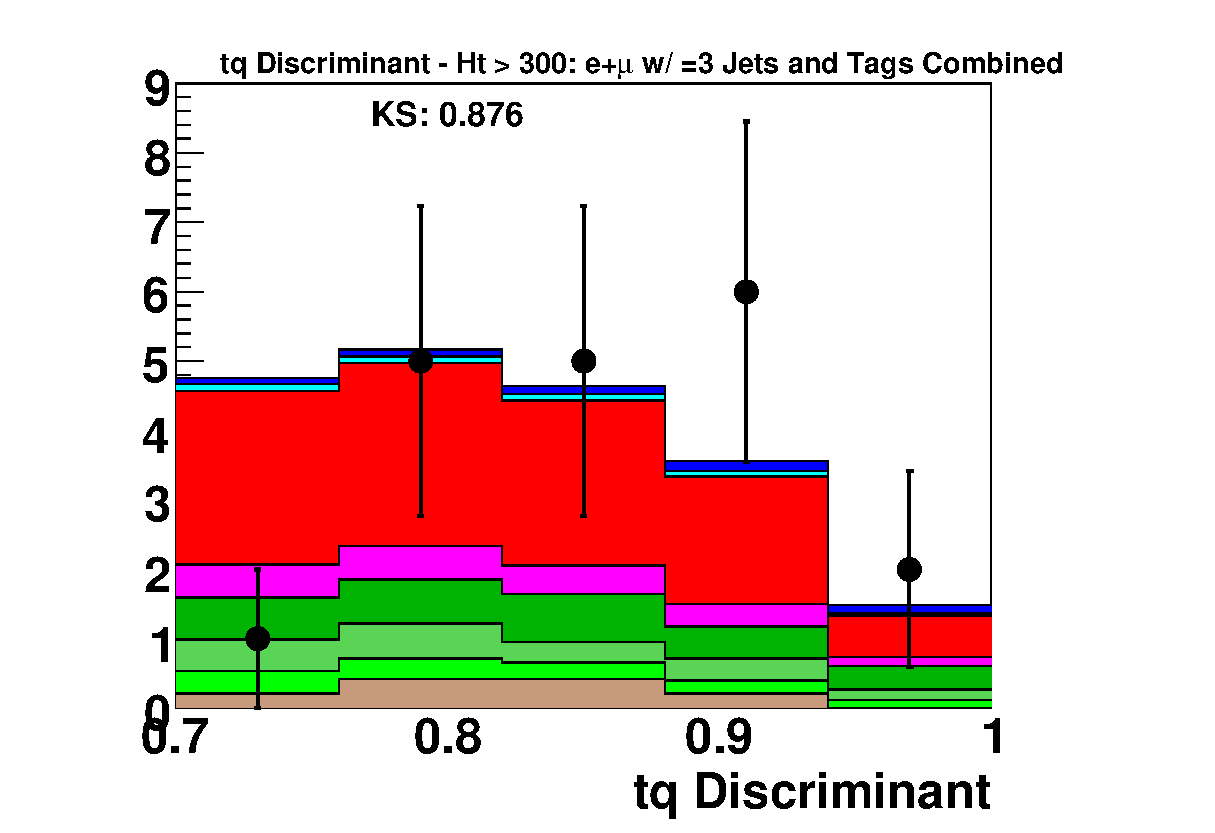
\includegraphics[width=0.40\textwidth]
{figures/cross_check/combined/3jet/TTbar_tq_Discriminant_Zoom}
\vspace{-0.1in}
\caption[ttbarcross]{``Hard $W$+jets'' cross-check plots in three-jet
events for the $tb$ discriminant (upper row) and the $tq$ discriminant
(lower row). The left column shows the full discriminant region while
the right column shows the high discriminant region above 0.7.}
\label{ttbar-cross-3jet}
\end{figure}

